\documentclass[aip,jcp,reprint,showkeys]{revtex4-1}

\usepackage{graphicx,bm,xcolor,hyperref,amsmath,amssymb,amsfonts,float}
\usepackage{hyperref}
\usepackage{algorithmicx}
\usepackage{algcompatible}
\usepackage{algpseudocode} 
\newcommand{\LeftComment}[1]{\State {\scriptsize /* \textit{#1} */}}

\usepackage{tikz,tikzscale}

\newcommand{\alert}[1]{\textcolor{red}{#1}}
\newcommand{\ket}[1]{|#1\rangle}
\newcommand{\stwo}{\hat{S}^2}
\newcommand{\tv}{\mathtt{v}}
\newcommand{\ttt}{\mathtt{t}}
\newcommand{\mb}{\mathtt{b}}
\newcommand{\md}{\mathtt{d}}
\newcommand{\mD}{\mathcal{D}}
\newcommand{\mpp}{\mathtt{p}}
\newcommand{\mpv}{\mathbf{p}}
\newcommand{\up}{\uparrow}
\newcommand{\dn}{\downarrow}
\newcommand{\Nint}{{N_\text{int}}}
\newcommand{\Norb}{{N_\text{orb}}}
\newcommand{\sop}{SOP}
\newcommand{\one}{{\texttt{1}}}
\newcommand{\zero}{{\texttt{0}}}



\begin{document}

\title{A fast algorithm to enforce spin-pure wave functions in selected configuration interaction}

% Kevin and Thomas : put the authors in the whatever order you prefer
% Kevin : Is your affiliation correct?
\author{Thomas Applencourt}
\author{Kevin Gasperich}
\affiliation{Argonne Leadership Computing Facility, Argonne National Laboratory, Argonne, Illinois 60439 USA}
\author{Anthony Scemama}
\affiliation{Laboratoire de Chimie et Physique Quantiques, Université de Toulouse, CNRS, UPS, France}

\begin{abstract}
\end{abstract}

\keywords{Selected Configuration Interaction ; Spin purity }

\maketitle

%----------------------------------------------------------------
\section{Introduction}
%----------------------------------------------------------------

In recent years, selected configuration interaction (sCI) methods have regained in
popularity,\cite{Greer_1998,Stampfuss_2005,Bytautas_2009,Booth_2009,Giner_2013,Buenker_2014,Holmes_2016,Ohtsuka_2017,Coe_2018}
especially for the accurate calculation of electronic excitation
energies.\cite{Coe_2013,Schriber_2017,Holmes_2017,Loos_2018,Scemama_2018,Dash_2018}
A balanced description of excited states requires the wave functions to be
spin-pure, i.e. eigenfunctions of the $\stwo$ operator.
A natural option would be to reformulate sCI in terms of configuration state
functions (CSF), but such a modification might increase the computational cost
of the selection procedure: for instance, with the CIPSI
selection\cite{Bender_1969,Whitten_1969,Huron_1973} the computation of the
perturbative contribution of a CSF would require the computation of all the
individual contributions of the determinants included in the CSF, which can
be large with many open shells.
In the context of heat-bath selection, Holmes \textit{et al} have proposed to
improve the spin purity of the wave functions by introducing ``time-reversal
symmetry''\cite{Holmes_2017}, which consists in exchanging the spin labels of
the electrons.
However, when the number of open shells is large, time-reversal symmetry is not
sufficient to generate all the required spin permutations among the open shells
which would generate all the determinants of the corresponding CSF.

Recently, Bytautas and Ruedenberg proposed a simple scheme to truncate large
spin-pure wave functions while keeping the spin-purity.\cite{Bytautas_2007}
By definition, all the determinants belonging to the same CSF have the same
\emph{spatial occupation pattern} (\sop), so the
coefficients of the determinants having the same {\sop}
are summed together to produce the so-called \emph{space-product
weights}, which are used to truncate the wave function. As spin coupling
coefficients are included in the CI expansion, the truncated wave function is
also an eigenfunction of $\stwo$.

Following this idea, imposing spin purity in sCI methods can be done by 
\begin{enumerate}
\item Identifying all the space occupation patterns of the determinants composing
      the variational space
\item Generating all the determinants (with imposed numbers of $\up$ and
      $\dn$ electrons) corresponding to these space occupation patterns
\item Diagonalizing the Hamiltonian in this expanded determinant space.
\end{enumerate}
An efficient algorithm to achieve this procedure is presented in this letter,
and was implemented in the \emph{Quantum Package}.\cite{qp}

%%%%%%%%%%%%%%%%%%%
\section{Algorithm}
%%%%%%%%%%%%%%%%%%%

Each Slater determinant $\mD_I$ is represented as a Waller-Hartree double
determinant,\cite{Pauncz_1989}
\begin{equation}
 \label{eq:di}
 \mD_I = D_i^\up \, D_j^\dn\, ,
\end{equation}
the product of a determinant of
$\up$ spinorbitals with a determinant of $\dn$ spinorbitals.
Such a representation can be encoded as a pair of bit strings $(\md_i,\md_j)$.
Within a bit string,
each bit corresponds to a spinorbital and the bit is set to \one{} when the
spinorbital is occupied. In low-level languages such as Fortran or C, a bit
string may be stored as an array of $\Nint$ 64-bit integers, where 
\begin{equation}
  \Nint = \left \lfloor \frac{\Norb-1}{64} \right \rfloor + 1,
\end{equation}
$\Norb$ being the number of molecular orbitals.
This representation
allows for efficient determinant comparisons using bit-wise operation 
capabilities of modern processors,\cite{Scemama_2013} and will be convenient
in the following.

All the CPU cycle measurements were performed  on an Intel(R) Xeon(R)
Gold 6140 CPU @ 2.30GHz with the GNU Fortran compiler 7.3.0, by reading
the time stamp counter of the CPU with the \texttt{rdtsc} instruction.


\subsection{Identification of the space occupation patterns}

The {\sop} $\mpv_I$ of determinant $\mD_I$ 
%defined in Eq.\eqref{eq:di}
is a vector of integers defined as
\begin{equation}
  [\mpv_I]_k = 
  \begin{cases} 
    0 & \text{when the $k$-th orbital is unoccupied} \\
    1 & \text{when the $k$-th orbital is singly occupied} \\
    2 & \text{when the $k$-th orbital is doubly occupied}
  \end{cases} 
\end{equation}
If $\mpv_I$ is encoded as a pair of bit strings $(\mpp_I^{(1)}, \mpp_I^{(2)})$, where
$\mpp_I^{(1)}$ encodes the singly occupied orbitals and where $\mpp_I^{(2)}$ the doubly
occupied orbitals, the {\sop} can be computed as
\begin{align}
\label{eq:sop}
  \mpp_I^{(1)} & = \md_i \oplus \md_j \\
  \mpp_I^{(2)} & = \md_i \wedge \md_j 
\end{align}
where $\oplus$ denotes the \texttt{xor} operator and $\wedge$ denotes the
\texttt{and} operator.

Transforming all the determinants into a list of unique \sop s can be done
in linear time, if a hash value is associated with each \sop .\cite{Bitton_1983}

\subsection{Generating all the determinants}

\begin{figure}[t]
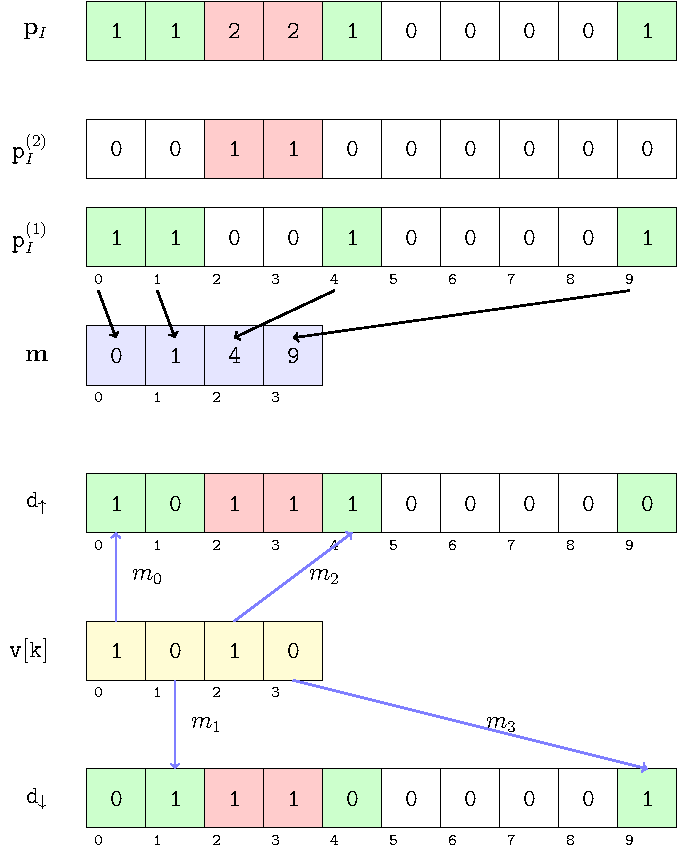
\includegraphics[width=0.9\columnwidth]{pattern.tikz} 
\caption{The SOP $\mpv_I$ is encoded as in Eq.~\eqref{eq:sop}. Singly and doubly
occupied orbitals are represented respectively in green and red.
The list of indices $\mathbf{m}$ of the singly occupied orbitals is built (in blue), and this
mapping is re-used to build the determinants from permutations generated by Anderson's algorithm (yellow).}
\label{fig:mapping}
\end{figure}


Given a {\sop}, one needs to generate all the possible excitations that can
occur in the singly occupied molecular orbitals, keeping the numbers of $\up$
and $\dn$ electrons fixed.
All the generated determinants will only differ by the singly occupied orbitals,
so from now on we will consider a more compact representation: a bit string of
$n_\up + n_\dn$ bits, where $n_\up$ and $n_\dn$ denote the number of $\up$ and
$\dn$ unpaired electrons.
To encode a determinant, if the orbital is occupied by an $\up$ electron the
corresponding bit will be set to \one{}, otherwise it will be set to \zero{}.

%where all the doubly occupied and unoccupied orbitals are removed, and keep
%the mapping from this compact representation to the full space of orbitals
%for the .

%One first extracts the list $l$ of unoccupied molecular
%orbital indices, and replaces the values in the list by 
%\one{} if the corresponding molecular orbital originates from the $\up$
%determinant, or \zero{} if it originates from the $\dn$ determinant. 
%This list is encoded in a bit string, and figure~\ref{fig:mapping} illustrates
%this mapping.


\begin{figure}[t]
\begin{algorithmic}
\Function{GenPermutations}{$n,m$}
  \LeftComment{$n$: Number of bits set to 1}
  \LeftComment{$m$: Number of bits set to 0}
  \LeftComment{$v$, $t$, $t'$, $t''$ and $p$ are encoded in at least $n+m+1$ bits}%
  \State $k \gets 0$
  \State $v \gets (1 \ll n) - 1$
  \State $p[0] \gets v$
  \While {$v < \left(1 \ll (n+m) \right) $}
    \State $k \gets k+1$
    \State $t \gets v \vee (v-1)$
    \State $t' \gets t + 1$\
    \State $t'' \gets \left((\neg t \wedge t')-1 \right) \gg (ctz(v)+1)$
    \State $p[k] \gets t' \vee t''$
  \EndWhile
  \State \Return $p$
\EndFunction
\end{algorithmic}
\caption{Anderson's algorithm to generate all the patterns of $n$ bits set to
$1$ in an integer of $n+m$ bits in lexicographic order.
$ctz$ counts the number of trailing zeros, 
$i \ll n$~: shifts $i$ $n$ bits to the left, 
$i \gg n$~: shifts $i$ $n$ bits to the right, 
$i \gg n$~: shifts $i$ $n$ bits to the right, 
$\wedge$~: bit-wise \texttt{and} operation, and
$\vee$~: bit-wise \texttt{or} operation}
\label{fig:algo}
\end{figure}

To generate all the determinants keeping the numbers of $\up$ and $\dn$
electrons constant, we need to build all the bit strings with $n_\up$
bits set to \one{} and $n_\dn$ bits set to \zero{}.
This compact representation allows us to use Anderson's algorithm\cite{NextBit},
which generates all
the patterns of $n_\up$ bits set to $1$ in a bit string of length $n_\up+n_\dn$
in lexicographical order. For example, with $n_\up=2$ and $n_\dn=2$
its generates \texttt{(0011, 0101, 0110, 1001, 1010, 1100)}.
The bit string $\tv$ is initialized with the smallest possible unsigned integer with
$n_\up$ bits set to \one, which is $2^{n_\up+1}-1$. Then, the
following steps are iterated until $\tv$ becomes greater than $2^{n_\up+n_\dn}-1$:
\begin{enumerate}
    \item Set all the least significant \zero{} bits of $\tv$ to \one{}, add \one{} and store the result in $\ttt$. The least significant \one{} of $\ttt$ marks the position in $\tv$ of the most significant \zero{} that should be changed into a \one{}.
    \item The position of the least significant \one{} of $\tv$ is identified by counting the number of trailing zeros in $\tv$. This \one{} should be changed into a \zero{}.
    \item At the right of this position, contiguous \one's should be added such that the total number of \one's stays unchanged.
\end{enumerate}
The corresponding pseudo-code is presented in Fig.~\ref{fig:algo}. On average, one loop cycle executes in only $8.2$~CPU cycles.

To build one generated determinant from a permutation, one needs to
\begin{itemize}
    \item 
\end{itemize}






%----------------------------------------------------------------
\section{Conclusion}
%----------------------------------------------------------------


%----------------------------------------------------------------
\begin{acknowledgments}
The authors gratefully acknowledge Sean Eron Anderson for creating the 
\emph{Bit Twiddling Hacks} web page.
This work was performed using HPC resources from CALMIP (Toulouse) under
allocations 2018-0510 and 2018-18005 and from GENCI-TGCC (Grant
2018-A0040801738).
\end{acknowledgments}

%----------------------------------------------------------------

\bibliography{s2}

\end{document}
